\section{Evaluation}
\label{sec:eval}

% P:eval-modelled
All results are modelled, and ratios above 1 favour CoDe.

\subsection{GEMM Speed and Area Efficiency}
\label{sec:eval:gemm}

% P:eval-gemm-summary
CoDe matches LP-Spec-style's GEMM speed on about half its logic and outruns P3-LLM-style once a GEMM has more than two
token rows. Fig.~\ref{fig:gemm} plots each design's GEMM speed-up over stock AiM and its GEMM throughput per logic
mm$^2$ against $M$, with the NPU's GEMM speed as a line; each point is the geometric mean over the FC shapes of
Section~\ref{sec:method:work}.

% P:eval-gemm-speed
\paragraph{GEMM speed}
Up to $M = 2$ the column period paces every design: one column read serves every token, and P3-LLM-style,
LP-Spec-style and CoDe all run 1.96--1.97$\times$ faster than stock AiM at $M = 2$ (Fig.~\ref{fig:gemm}a). From
$M = 3$ P3-LLM-style needs a second pass for the tokens beyond its two per read, while CoDe fills up to four beats per
command: at $M = D = 4$ CoDe runs 3.74$\times$ stock AiM's speed on the mobile platform and 3.82$\times$ on the edge
server, against P3-LLM-style's 1.95$\times$. LP-Spec-style also fills four beats per column period, with four times
the multipliers, so its curve coincides with CoDe's up to $M = 4$, and at every $M$ on the edge server, where CoDe's
tile of $V = D = 4$ issues LP-Spec-style's command stream. On the mobile platform CoDe's eight-token tile also covers
$M = 5$--8 in one row sweep where LP-Spec-style needs a second pass, and CoDe runs 1.62$\times$ LP-Spec-style's speed
at $M = 5$.

% P:eval-gemm-per-mm2
\paragraph{GEMM throughput per logic mm$^2$}
Per logic mm$^2$, CoDe nearly doubles LP-Spec-style's GEMM throughput on both platforms. CoDe fills the same beats as
LP-Spec-style but spends its logic on storage rather than multipliers, so it reaches LP-Spec-style's speed with
0.539$\times$ its logic area on the mobile platform and 0.56$\times$ on the edge server
(Section~\ref{sec:method:designs}). CoDe therefore returns 1.86$\times$ LP-Spec-style's GEMM throughput per logic
mm$^2$ on the mobile platform up to $M = 4$ and 1.99--2.07$\times$ from $M = 8$, with a peak of 3.01$\times$ at
$M = 5$, where LP-Spec-style runs its second pass; on the edge server the ratio is 1.79$\times$ at every $M$
(Fig.~\ref{fig:gemm}b). Against P3-LLM-style, CoDe's speed outgrows its larger logic from $M = 3$: CoDe returns
1.43$\times$ P3-LLM-style's throughput per logic mm$^2$ at $M = 4$ and 1.53--1.59$\times$ from $M = 8$ on the mobile
platform, and 1.46--1.48$\times$ at $M = 3$--4 and from $M = 8$ on the edge server. Only at $M \le 2$, where CoDe's
third and fourth beats sit idle, does P3-LLM-style's smaller PU lead, with CoDe at 0.75$\times$.

% figure* (Section VI-B): placement checked on the float map after each build
\begin{figure*}[t]
  \centering
  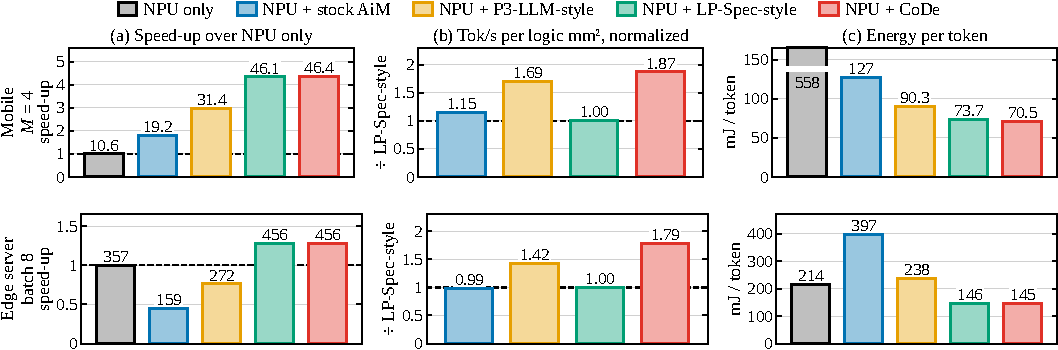
\includegraphics[width=\textwidth]{figs/fig_e2e.pdf}
  \caption{End-to-end decoding, mobile platform (top) and edge server (bottom): (a)~speed-up over NPU only, tokens/s
  on bars; (b)~tokens/s per logic mm$^2$; (c)~energy per token.}
  \label{fig:e2e}
\end{figure*}

\subsection{End-to-End Speedup}
\label{sec:eval:e2e}

% P:eval-e2e-phone
\paragraph{Mobile platform}
Fig.~\ref{fig:e2e} runs whole decoding on the five systems of Section~\ref{sec:method:work}: the speculative loop at
$M = 4$ on the mobile platform and a batch of 8 on the edge server. On the mobile platform CoDe and LP-Spec-style
decode fastest, 4.37$\times$ and 4.34$\times$ faster than NPU only, at 46.4 and 46.1 tokens/s
(Fig.~\ref{fig:e2e}a). P3-LLM-style reaches 2.96$\times$, because its two-token read needs two passes over the four
token rows, and stock AiM reaches 1.81$\times$. At each system's own best $M$ the order holds: CoDe reaches
47.1 tokens/s and LP-Spec-style 46.8 at $M = 3$, P3-LLM-style 43.8 and stock AiM 26.5 at $M = 2$, and NPU only 10.6
at $M = 4$. Past $M = 4$ CoDe's eight-token tile pulls ahead: CoDe's loop runs 1.31$\times$ faster than
LP-Spec-style's at $M = 5$ and 1.05--1.31$\times$ faster over $M = 5$--16.

% P:eval-e2e-server
\paragraph{Edge server}
On the edge server only CoDe and LP-Spec-style decode a batch of 8 faster than NPU only, both 1.28$\times$ at
456 tokens/s (Fig.~\ref{fig:e2e}a). Stock AiM runs at 0.45$\times$ and P3-LLM-style at 0.76$\times$ NPU only's speed,
so at the batch where P3-LLM~\cite{p3llm} moves its linear layers to the NPU, CoDe decodes 1.68$\times$ faster than
P3-LLM-style. On the geometric mean over the five models, NPU only overtakes CoDe from batch 16.

% P:eval-e2e-per-mm2
\paragraph{Throughput per logic mm$^2$}
At LP-Spec-style's decoding speed, CoDe nearly doubles LP-Spec-style's tokens per second per logic mm$^2$ on both
platforms. CoDe returns 1.87$\times$ LP-Spec-style's decoding throughput per logic mm$^2$ on the mobile platform and
1.79$\times$ on the edge server (Fig.~\ref{fig:e2e}b), because CoDe matches LP-Spec-style's speed on about half its
logic. Against P3-LLM-style, whose PU takes less logic than CoDe's, CoDe's speed lead more than repays the area:
CoDe returns 1.10$\times$ P3-LLM-style's decoding throughput per logic mm$^2$ on the mobile platform and 1.26$\times$ on the
edge server.

\subsection{Energy and Peak Power}
\label{sec:eval:energy}

% P:eval-energy
\paragraph{Energy per token}
CoDe spends the least energy per token of the five systems on both platforms. On the mobile platform the speculative
loop on CoDe spends 70.5\,mJ per token at $M = 4$, while NPU only spends 7.9$\times$, stock AiM 1.80$\times$,
P3-LLM-style 1.28$\times$ and LP-Spec-style 1.04$\times$ CoDe's energy (Fig.~\ref{fig:e2e}c). On the edge server,
with the NPU idling at 55\,W while the PIM works, NPU only spends 1.48$\times$ and P3-LLM-style 1.64$\times$ CoDe's
energy per token, and LP-Spec-style ties CoDe; with the idle NPU power-gated, P3-LLM-style still spends 1.46$\times$
CoDe's energy.

% P:eval-power
\paragraph{Peak power}
CoDe's faster PU clock keeps its peak power within a few percent of LP-Spec-style's, and each of its clock edges
draws less charge. With every PU at its full MAC rate, CoDe draws 1.04$\times$ LP-Spec-style's peak power per die on
the mobile platform and 1.03$\times$ per pseudo-channel on HBM2 (Table~\ref{tab:params}); stock AiM and P3-LLM-style
draw less because they run fewer MACs per column period. CoDe spreads the same MAC rate over four times as many clock
edges: its PUs switch 522\,pJ per die every 1.25\,ns against LP-Spec-style's 1,776\,pJ every 5\,ns, so each CoDe edge
draws 3.4$\times$ less charge, and 3.1$\times$ less on HBM2, which lowers the current step that the die's power grid
absorbs. Clock gates on CoDe's mostly idle accumulator slots and staging words would cut its peak power to
0.92$\times$ and 0.87$\times$ ungated LP-Spec-style's; every other number describes the ungated designs.

\subsection{Ablation Study}
\label{sec:eval:ablation}

% P:eval-gain-sources
\paragraph{Sources of CoDe's gain}
CoDe's gain over stock AiM has two sources, row reuse and beat filling, and each source is worth more once the other
is present. Table~\ref{tab:umac_src} adds the two sources with row reuse first for one decoder layer's weight GEMMs at $M = 8$, the layer of Table~\ref{tab:umac} on the mobile platform and
of Llama-3.1-8B on the edge server. The row-reuse-only design keeps the stock PU's pace of one beat per column
period and adds CoDe's storage and row sweeps of $V$ tokens; we simulate it as CoDe's trace at $D = 1$. Row reuse alone speeds
the layer up 1.24$\times$ on the mobile platform and 1.15$\times$ on the edge server, yet $U$ reaches only 0.223 and
0.222, because \UMAC stays at 1/4.
Beat filling, the command decoupling of Section~\ref{sec:design:beat}, then fills the idle beats and supplies the large step,
3.49$\times$ on the mobile platform and 3.33$\times$ on the edge server, while CoDe's \fMAC of 0.779 and 0.739 stays
near stock AiM's 0.717 and 0.771. In the other order, which we model as a quarter of stock AiM's MAC slots plus its non-MAC time per row sweep rather
than simulate, beat filling alone would cut \fMAC,
and with \UMAC at 1 also $U$, to 0.425 and 0.506, in steps of 2.37$\times$ then 1.83$\times$ on the mobile platform
and 2.62$\times$ then 1.46$\times$ on the edge server: the unchanged non-MAC commands would take more than half of the
shortened time on the mobile platform and about half on the edge server. Beat filling thus earns its full step only
once row reuse has removed most of the row-switch overhead per token.

% P:eval-vsweep-summary
\paragraph{Choice of tile size}
Throughput per logic mm$^2$ peaks at the tile size $V = D$ on both platforms, and the mobile platform's $V = 8$
bounds the per-mm$^2$ loss across the token rows of a decode step. Fig.~\ref{fig:vsweep}a sweeps $V$ from 1 to 64 for
q\_proj at $M = 64$ with the staging of Section~\ref{sec:design:pu}, which on the mobile platform is a register of
$V$ slices below $V = 8$; Fig.~\ref{fig:vsweep}b sets $V = 8$ against $V = 4$ for $M = 1$--16.

% P:eval-vsweep-gain
\paragraph{Gain by tile size}
Up to $V = D$ a larger tile fills idle beats; beyond $V = D$ it removes only row-switch commands. CoDe's q\_proj
speed-up over stock AiM rises from 1 at $V = 1$ to 3.86$\times$ on the mobile platform and 3.69$\times$ on HBM2 at
$V = D$, but only to 4.90$\times$ and 4.39$\times$ at $V = 64$. On the mobile platform, of the time that the step from
$V = 1$ to 2 saves, idle beats supply 72\,\%, row-switch commands 21\,\% and refresh 7\,\%. From $V = 4$ to 8 the
row-switch commands supply 91.6\,\% of the saving, and their share of the GEMM time falls from 18.9\,\% to 10.4\,\%;
token load stays at 20.5\,$\mu$s at every $V$.

% P:eval-vsweep-area
\paragraph{Area against speed}
Past $V = D$ CoDe's storage grows faster than its speed. Fig.~\ref{fig:vsweep}a normalises throughput per logic
mm$^2$ to stock AiM's, and both per-mm$^2$ curves peak at $V = D$, at 3.01$\times$ on the mobile platform and
2.34$\times$ on HBM2. From $V = 4$ to 8 the mobile
logic grows by 16\,\%, from 1.212 to 1.406\,mm$^2$ per die, and HBM2's by 40\,\%, from 0.821 to 1.153\,mm$^2$ per
pseudo-channel, so $V = 8$ breaks even per mm$^2$ only at 1.160$\times$ and 1.405$\times$ $V = 4$'s speed. At
$M = 64$, $V = 8$ runs 1.117$\times$ and 1.089$\times$ faster and keeps 96.3\,\% and 77.5\,\% of the peak.

% P:eval-vsweep-robust
\paragraph{Robustness across $M$}
Partial last row sweeps make $V = 8$ win per mm$^2$ on the mobile platform at $M = 5$--7, 9--10 and 13--15. At
$M = 5$, $V = 4$ runs two row sweeps of three and two tokens where $V = 8$ runs one, and $V = 8$'s verify step
returns 1.324$\times$ $V = 4$'s throughput per mm$^2$; up to $M = 4$ both tiles run one row sweep and $V = 8$ returns
0.862$\times$ (Fig.~\ref{fig:vsweep}b). HBM2's batched step never reaches the 1.405$\times$ break-even, and $V = 8$
peaks at 0.944$\times$ at $M = 5$. Against the best of $V = 2$, 4, 8 and 16 at each $M$ from 3 to 16, the mobile
$V = 4$'s worst per-mm$^2$ loss is 29.4\,\% on q\_proj and 24.5\,\% on the verify step, both at $M = 5$, while
$V = 8$'s is 13.8\,\%, its area premium at $M = 3$--4. On HBM2, $V = 4$ loses at most 11.7\,\% and $V = 8$
loses 28.8--30.0\,\%. The mobile one-tile kernel is the exception, because its single GB fill serves one row sweep and token load
takes 28.3\,\% of stock AiM's time at $M = 8$ (Fig.~\ref{fig:breakdown}): it loses 4.6\,\% with $V = 4$ and
13.8\,\% with $V = 8$. The speculative loop's best $M$ is 3 with the 1.1B draft and 4 with EAGLE, where $V = 8$ pays
its area premium; CoDe still sets $V = 8$ on the mobile platform, because $V = 8$ caps the per-mm$^2$ loss at 13.8\,\%
over $M = 3$--16, against $V = 4$'s 29.4\,\%.

% Fig. vsweep: one column; placement checked on the float map after each build
\begin{figure}[t]
  \centering
  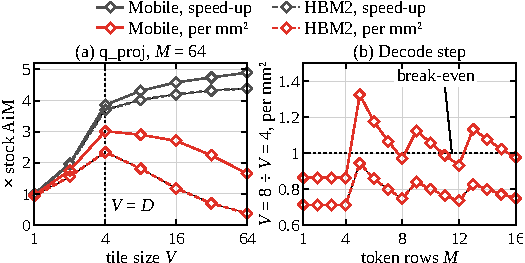
\includegraphics[width=\columnwidth]{figs/fig_vsweep.pdf}
  \caption{Tile size: (a)~q\_proj speed-up and throughput per logic mm$^2$ over stock AiM against $V$ at $M = 64$; (b)~$V = 8$ over
  $V = 4$, decode-step throughput per logic mm$^2$ against $M$.}
  \label{fig:vsweep}
\end{figure}

% sources-of-gain table (D-35; generated by scripts/make_tables.py, simulated rows, evaluation/dac_2x2 Sec. 2i):
% placement checked on the float map after each build
\begin{table}[t]
  \caption{Useful-MAC utilization from stock AiM to CoDe, one source at a time.}
  \label{tab:umac_src}
  \centering
  \footnotesize
  \setlength{\tabcolsep}{4pt}
  % generated by scripts/make_tables.py from evaluation/dac_2x2/figures/tab_umac_src_steps.csv (usrc_steps ids, simulated rows, layer, M = 8); do not edit
\begin{tabular}{@{}lccccc@{}}
\toprule
Design & \UMAC & \fMAC & $U$ & \multicolumn{2}{c@{}}{Speedup} \\
\cmidrule(l){5-6}
 & & & & step & cumul. \\
\midrule
\multicolumn{6}{@{}l}{\emph{Mobile:} Llama-2-7B, $V = 8$} \\
Stock AiM & 0.25 & 0.776 & 0.194 & -- & 1.00 \\
Row reuse only & 0.25 & 0.965 & 0.241 & 1.24 & 1.24 \\
\textbf{CoDe} & 1.00 & 0.843 & 0.843 & 3.49 & 4.35 \\
\midrule
\multicolumn{6}{@{}l}{\emph{Server:} Llama-3.1-8B, $V = 4$} \\
Stock AiM & 0.25 & 0.771 & 0.193 & -- & 1.00 \\
Row reuse only & 0.25 & 0.887 & 0.222 & 1.15 & 1.15 \\
\textbf{CoDe} & 1.00 & 0.739 & 0.739 & 3.33 & 3.83 \\
\bottomrule
\end{tabular}

\end{table}
